
\documentclass[border=8pt, multi, tikz]{standalone}
\usepackage{import}
\usepackage{graphicx}
\subimport{../layers/}{init}
\usetikzlibrary{positioning}
\usetikzlibrary{3d} %for including external image

\def\ConvColor{rgb:yellow,5;red,2.5;white,5}
\def\ConvReluColor{rgb:yellow,5;red,5;white,5}
\def\PoolColor{rgb:red,1;black,0.3}
\def\UpsampleColor{rgb:green,5; white,2}
\def\DetectColor{rgb:red,5; white,2}
\def\UnpoolColor{rgb:blue,2;green,1;black,0.3}
\def\FcColor{rgb:blue,5;red,2.5;white,5}
\def\FcReluColor{rgb:blue,5;red,5;white,4}
\def\SoftmaxColor{rgb:magenta,5;black,7}
\def\SumColor{rgb:green, 1}
\def\ShortcutColor{rgb: blue, 3; green, 1; white, 5}
\def\MultColor{rgb: magenta, 1}
\def\ConcColor{rgb:red, 5}
\def\input_image{../examples/stop_sign.jpg}

\newcommand{\copymidarrow}{\tikz \draw[-Stealth,line width=0.8mm,draw={rgb:blue,4;red,1;green,1;black,3}] (-0.3,0) -- ++ (0.3,0);}

\begin{document}
\begin{tikzpicture}
\tikzstyle{connection}=[ultra thick,every node/.style={sloped,allow upside down},draw=\edgecolor,opacity=0.7]
\tikzstyle{copyconnection}=[ultra thick,every node/.style={sloped,allow upside down},draw={rgb:blue,4;red,1;green,1;black,3},opacity=0.7]

\node[canvas is zy plane at x=0] (image_0) at (-4,0,0) {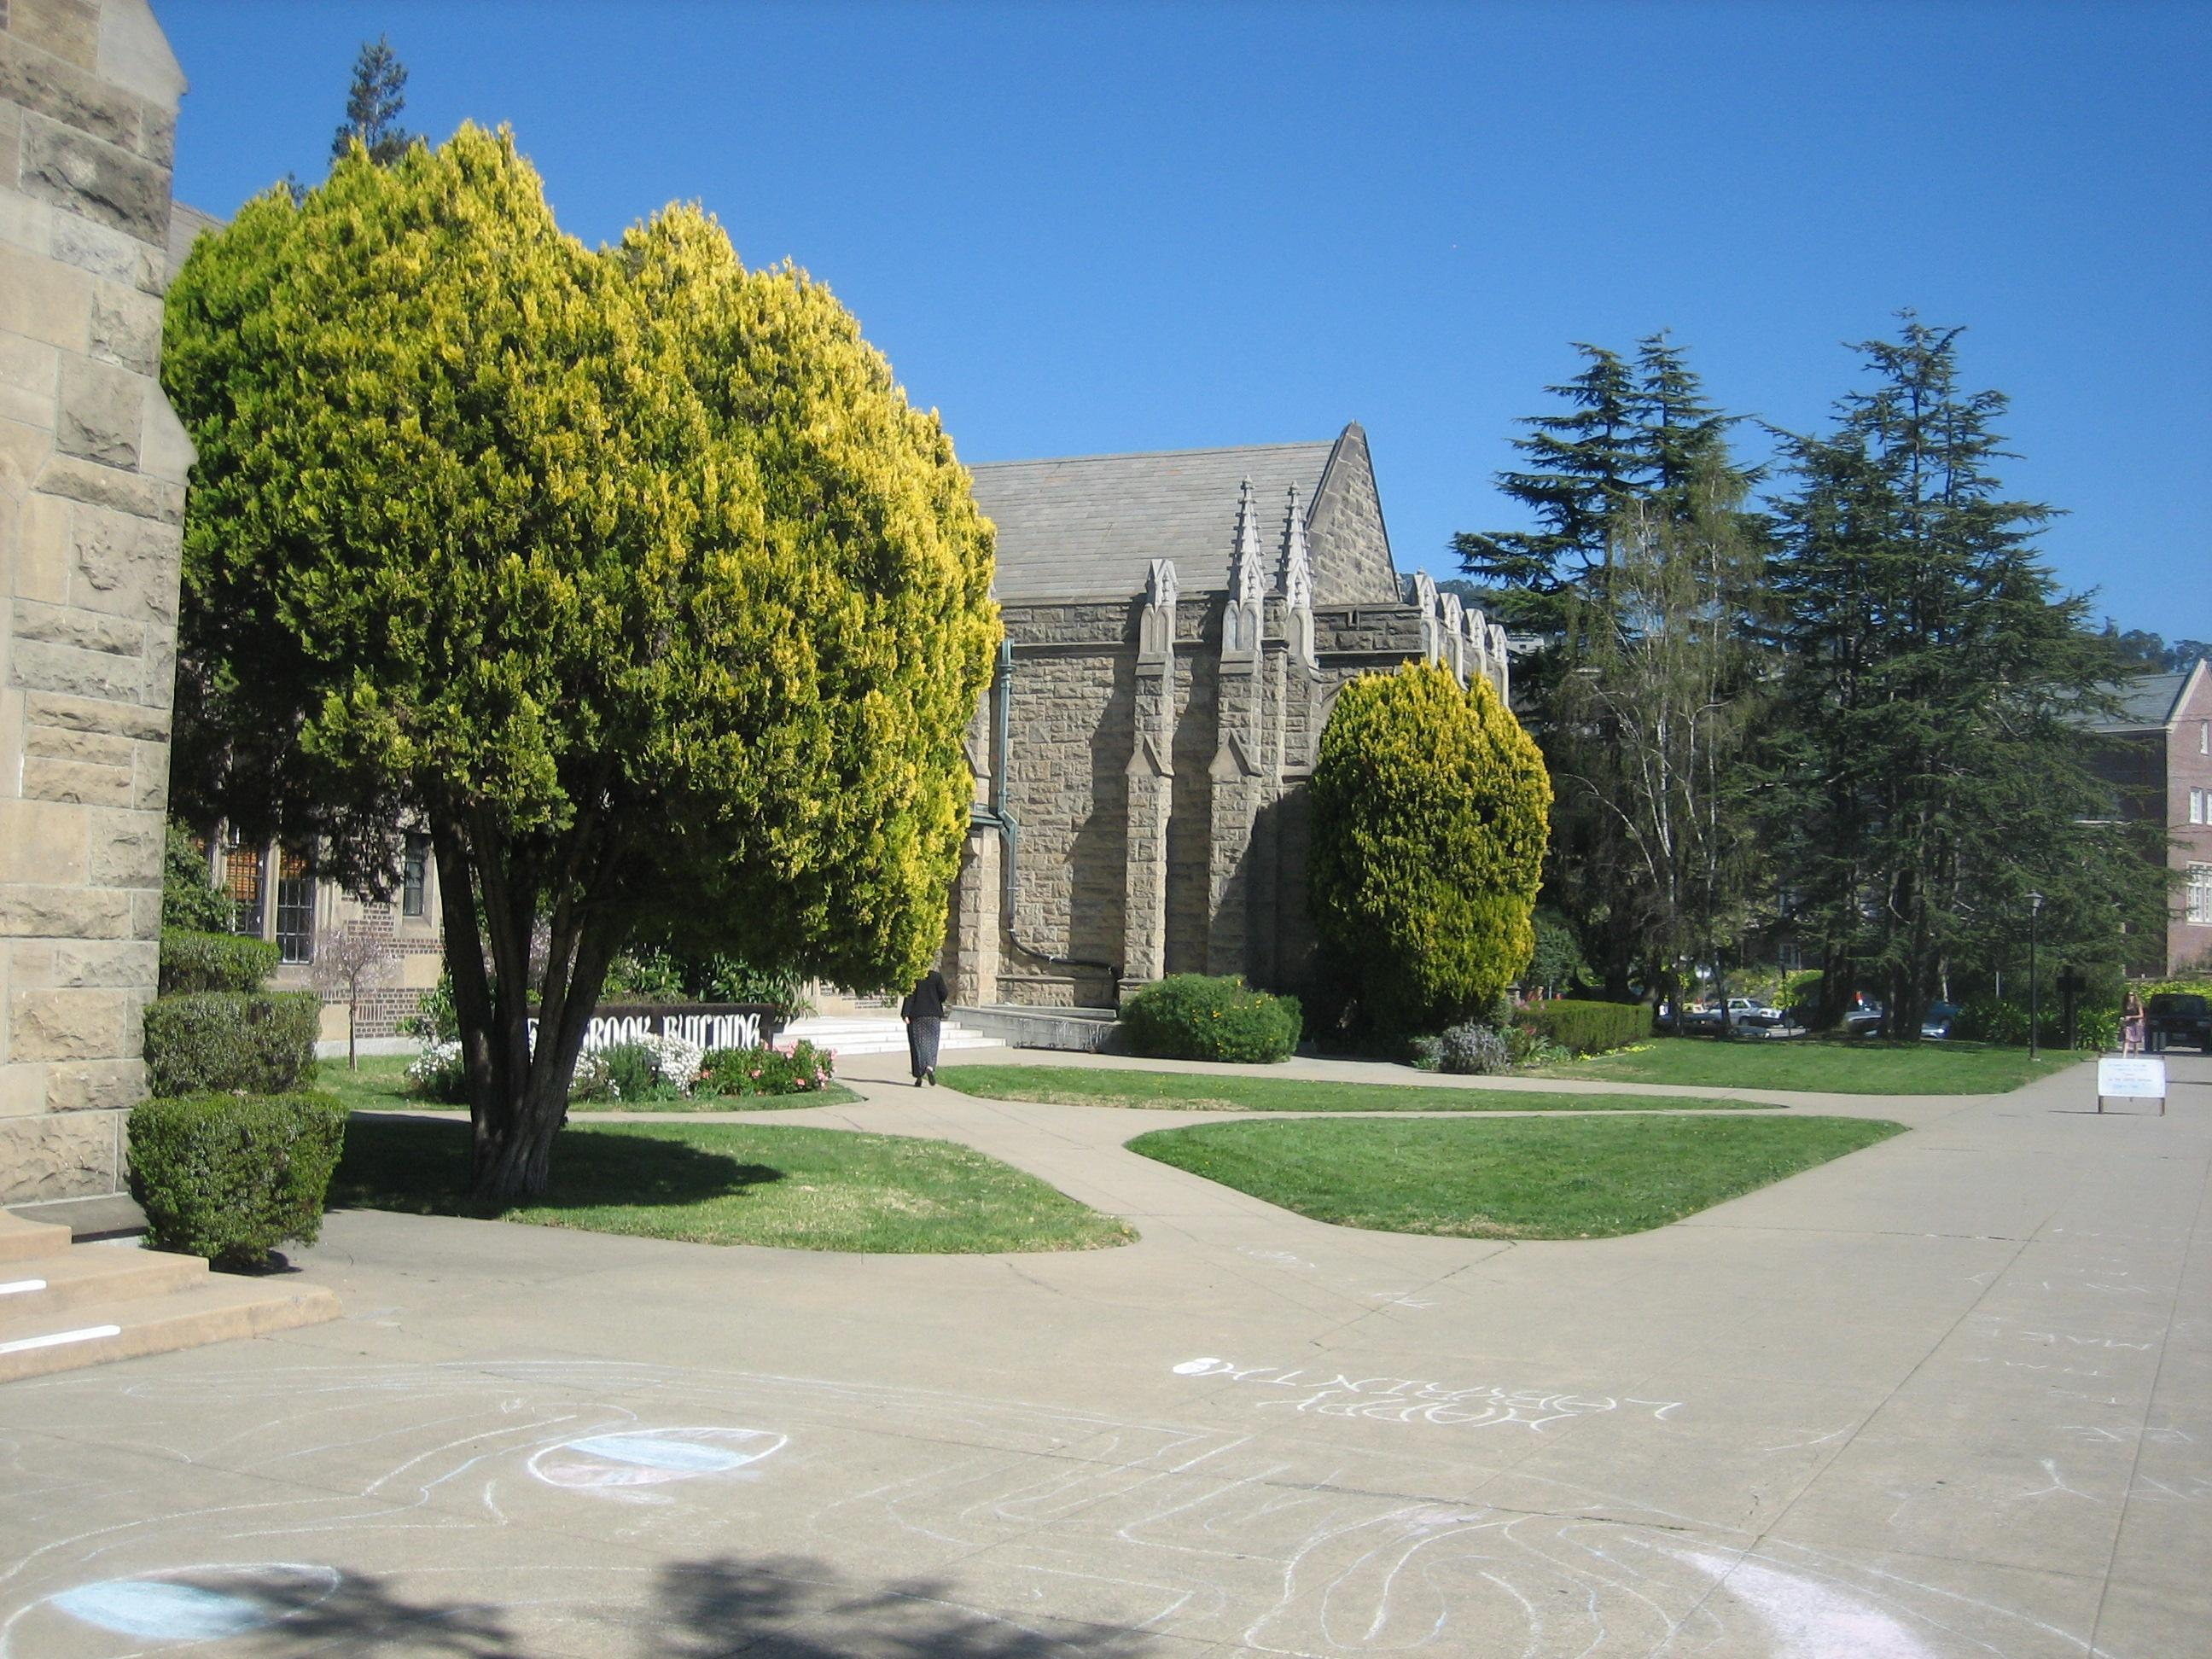
\includegraphics[width=10cm ,height=10cm ]{\input_image}};

\pic[shift={(1, 0, 0)}] at (0,0,0)
    {RightBandedBox={
        name=conv_0,
        caption=,
        xlabel={(64,)},
        zlabel=256,
        fill=\ConvColor,
        bandfill=\ConvReluColor,
        height=32,
        depth=32,
        width={3.0}
        }
    };

\end{tikzpicture}
\end{document}
